The most dominant dynamics of a refridgeration container/trailer are thermal dynamics of the metal in heat exchangers (i.e. evaporator and condensor). Some components in the system will have dynamics so much faster than the dominant dynamics that they will be considered static (compressor and expansion valves).
In the end the model will be composed of a model that represents the refridgeration cycle along with a model of the thermal masses (in heat exchangers, other metal parts and cargo)


\subsection{Component models}

\subsubsection{General type refrigerant control volume state eq}
Many of the components in a refridgeration cycle will be based on similar state equations. They will generally express the change in mass inside the control volume and/or the specific enthalpy out of the control volume. These can be constructed from the mass conservation equation and the energy balance equation of the control volume.

\textbf{Mass conservation equation} \\
\begin{equation} \label{eq:GeneralTypeControlVol_MassConservation}
	\frac{dM}{dt} = \dot{m_{in}} - \dot{m_{out}}
\end{equation}

where 
\begin{center}
	\begin{tabular}{l p{8cm} l}
		$\frac{dM}{dt}$ & is the change in mass inside control volume & [\si{kg}/\si{s}]\\ 
		$\dot{m_{in}}$ & flow into control volume & [\si{kg}/\si{s}]\\
		$\dot{m_{out}}$ & flow out of control volume & [\si{kg}/\si{s}]\\
	\end{tabular}
\end{center}

\textbf{Energy balance equation}
\begin{equation}
	h_{out} = h_{in} + \frac{Q_{in}}{\dot{m}_{in}}
\end{equation}

where
\begin{center}
	\begin{tabular}{l p{8cm} l}
		$h_{out}$ & specific enthalpy out of the control volume & [\si{J}/\si{kg}]\\ 
		$h_{in}$ & specific enthalpy into control volume & [\si{J}/\si{kg}]\\ 
		$Q_{in}$ & energy flow applied to control volume& [\si{W}]\\
		$\dot{m}_{in}$ & flow into control volume & [\si{kg}/\si{s}]\\
	\end{tabular}
\end{center}

\subsubsection{Expansion valve}
The flow through an expansion valve is proportional to the square root of the pressure drop across it, where the proportional constants relies on physical properties of the valve and refrigerant.
\begin{equation} \label{eq:ExpansionValve}
	\dot{m}= C A \sqrt{\rho\Delta p}
\end{equation}

where 
\begin{center}
	\begin{tabular}{l p{8cm} l}
		$\dot{m}$ & flow through valve & [\si{kg}/\si{s}]\\ 
		$\Delta p$ & pressure drop across valve & [\si{Pa}]\\
		$C$ & discharge coefficient of valve & [$\cdot$]\\
		$A$ & cross sectional area of valve & [\si{m^2}]\\
		$\rho$ & density of liquid & [\si{kg}/\si{m^3}]\\
		$C$ & discharge coefficient of valve & [$\cdot$]\\
	\end{tabular}
\end{center}

To model the way that the valve is intended to be controlled, an alternative representation is introduced for the mass flow through an expansion valve \cref{eq:ExpansionValve_DutyCycle}

\begin{equation} \label{eq:ExpansionValve_DutyCycle}
	\dot{m}= D_{on} K  \sqrt{\frac{1}{v_{in} (p_{in} - p_{out})}}
\end{equation}

where 
\begin{center}
	\begin{tabular}{l p{8cm} l}
		$\dot{m}$ & flow through valve & [\si{kg}/\si{s}]\\ 
		$D_{on}$ & fraction of each pulse period being on & [$\%$]\\
		$p_{in}$ & absolute pressure on input side & [\si{Pa}]\\
		$K$ & $C A$ & [\si{m^2}]\\
		$v_{in}$ & specific volume of liquid & [\si{m^3}/\si{kg}]\\
		$p_{out}$ & absolute pressure on output side & [\si{Pa}]\\
	\end{tabular}
\end{center}

\subsubsection{Pipe Joining Junction} 
Between compressor $ C_1 $, $ C_2 $ and the economizer (see \cref{fig:HVAC_Diagram}) is a Pipe Joining Junction that connects the three forementioned components.

\begin{equation} \label{eq:PipeJoiningJunction_ChangeOfMass}
	\frac{dM}{dt} = \dot{m}_{in1} + \dot{m}_{in2} + \dot{m}_{out}
\end{equation}

where 

\begin{center}
	\begin{tabular}{l p{8cm} l}
		$\frac{dM}{dt}$ & is the change in mass inside Pipe Joining Junction		 	& [\si{kg}/\si{s}]\\ 
		$\dot{m}_{in1}$ & flow into Pipe Joining Junction from Compressor $ C_1 $ 		& [\si{kg}/\si{s}]\\
		$\dot{m}_{in2}$ & flow into Pipe Joining Junction from Economiser 				& [\si{kg}/\si{s}]\\
		$\dot{m_{out}}$ & flow into Compressor $ C_2 $ from Pipe Joining Junction		& [\si{kg}/\si{s}]\\
	\end{tabular}
\end{center}

In \cref{eq:PipeJoiningJunction_ChangeOfMass}, the change of mass inside the Pipe Joining Junction can be expressed as a function of the mass flows into and out of the Pipe Joining Junction. 

\begin{equation} \label{eq:PipeJoiningJunction_Enthalpy}
	h_{out} = \frac{h_{in1} \cdot \dot{m}_{in1} + h_{in2} \cdot \dot{m}_{in2}}{ \dot{m}_{in1} + \dot{m}_{in2} }
\end{equation}

where

\begin{center}
	\begin{tabular}{l p{10cm} l}
		$h_{out}$ 	& specific enthalpy into Compressor $ C_2 $ from Pipe Joining Junction 		& [\si{J}/\si{kg}]\\ 
		$h_{in1}$ 	& specific enthalpy into Pipe Joining Junction from Compressor $ C_1 $  		& [\si{J}/\si{kg}]\\ 
		$h_{in2}$ 	& specific enthalpy into Pipe Joining Junction from Economiser   			& [\si{J}/\si{kg}]\\ 
		$\dot{m}_{in1}$ & flow into Pipe Joining Junction from Compressor $ C_1 $ 		& [\si{kg}/\si{s}]\\
		$\dot{m}_{in2}$ & flow into Pipe Joining Junction from Economiser 				& [\si{kg}/\si{s}]\\
	\end{tabular}
\end{center}
In \cref{eq:PipeJoiningJunction_Enthalpy} the specific enthalpy of the flow out of the Pipe Joining Junction is expressed as a function of the input flows and enthalpies. This equation is based on the energy balance, assuming no heat transfer to surroundings, i.e. the Pipe Joining Junction is perfectly insulated.

\subsubsection{Pipe Splitting Junction}

This component is particularly simple, as the only function of it is to split the input flow in two. It is furthermore assumed that the dynamics are fast enough that the they can be modelled as algebraic equations.

\begin{equation} \label{eq:PipeSplittingJunction_Enthalpy}
	\begin{split}
		\dot{m}_{in} &= \dot{m}_{out1} + \dot{m}_{out2} \\
		p_{out1} &= p_{in} \\
		p_{out2} &= p_{in} \\
		h_{out1} &= h_{in} \\
		h_{out1} &= h_{in} \\
	\end{split}
\end{equation}

where

\begin{center}
	\begin{tabular}{l p{12cm} l}
		$\dot{m}_{in}$ 		& mass flow into Pipe Splitting Junction from Condenser (reciever?) 						& [\si{kg}/\si{s}]\\
		$\dot{m}_{out1}$ 	& mass flow into Economiser expansion valve from Pipe Splitting Junction 				& [\si{kg}/\si{s}]\\
		$\dot{m}_{out2}$ 	& mass flow into Economiser heat exchanger from Pipe Splitting Junction 					& [\si{kg}/\si{s}]\\
		$p_{in}$ 			& absolute pressure input Pipe Splitting Junction from Condenser (reciever?)		& [\si{Pa}]\\
		$p_{out1}$ 			& absolute pressure into Economiser expansion valve from Pipe Splitting Junction 	& [\si{Pa}]\\
		$p_{out2}$ 			& absolute pressure into Economiser heat exchanger from Pipe Splitting Junction 	& [\si{Pa}]\\
		$h_{in}$ 			& specific enthalpy into Pipe Splitting Junction from Condenser (reciever?)   		& [\si{J}/\si{kg}]\\ 
		$h_{out1}$ 			& specific enthalpy into Economiser expansion valve from Pipe Splitting Junction	& [\si{J}/\si{kg}]\\ 
		$h_{out2}$ 			& specific enthalpy into Economiser heat exchanger from Pipe Splitting Junction		& [\si{J}/\si{kg}]\\ 
	\end{tabular}
\end{center}


The pressure and enthalpy on the output flows are equal to the input pressure and enthalpy. The sum of the mass flows out of the Pipe Splitting Junction is equal to the input mass flow. \\

\subsubsection{Compressor}
The compressor in the refrigeration cycle consists of two compressor stages that can be described by the same equations.
The compressor dynamics are assumed to be fast enough compared with the refridgeration cycle that it can be considered constant. Therefore, the equations governing the compressors are algebraic equations. 
Adiabatic compression is assumed. 
The two equations describing the compression governs the mass flow and the output enthalpy. The output enthalpy is found via a lookup table (HTP). 

\begin{align}
	\dot{m} &= \left(\frac{V_1}{v_1} - \frac{V_C}{v_2}\right) \frac{\omega}{2} \\
	h_{out} &= HTP(T_{out}, p_{out}) 
\end{align}

where

\begin{center}
	\begin{tabular}{l p{8cm} l}
		$\dot{m}$				& flow through compressor stage					& [\si{kg}/\si{s}]\\ 
		$h_{out}$				& compressor stage output enthalpy				& [\si{J}/\si{kg}]\\ 
		$V_1$					& cylinder internal volume b.f. stroke			& [$\si{m}^3$]\\ 
		$V_C$					& cylinder clearance volume after stroke		& [$\si{m}^3$]\\ 
		$v_1$					& refrigerant specific volume b.f. stroke		& [$\si{m}^3/\si{kg}$]\\
		$v_2$					& refrigerant specific volume after stroke		& [$\si{m}^3/\si{kg}$]\\
		$\omega$ 				& compressor angular velocity 					& [\si{rad}/\si{s}]\\
		$T_{out}$ 				& compressor stage output temperature 			& [\si{K}]\\
		$p_{out}$				& compressor stage output pressure 				& [\si{Pa}]\\
	\end{tabular}
\end{center}

\begin{align}
	v_2 &= \left(\frac{p_2}{p_1}\right)^{\frac{-1}{\gamma}} \\
	p_1 &= p_{in} - kl_1 \cdot \omega \\
	p_2 &= p_{out} + kl_2 \cdot \omega \\
	\gamma &= C_{cp}/C_{cv} \\
	T_{out} &= T_{in}\cdot \left(\frac{p_{out}}{p_{in}}\right)^{\frac{\gamma-1}{\gamma}}
\end{align}

where 

\begin{center}
	\begin{tabular}{l p{8cm} l}
		$p_{in}$				& compressor stage input pressure 			& [\si{Pa}]\\
		$p_1$					& piston input pressure									& [\si{Pa}]\\ 
		$p_2$					& piston output (discharge) pressure 		& [\si{Pa}]\\ 
		$\gamma$				& heat capacity ratio 								& [$ \cdot $]\\
		$ kl_1$, $kl_2$			& valve loss constants							& [$ \cdot $]\\
		$\omega$ 				& compressor angular velocity 				& [\si{rad}/\si{s}]\\
		$T_{in}$ 				& compressor stage input temperature 	& [\si{K}]\\
		$C_{cp}$ 				& Specific heat capacity - constant pressure 	& [\si{J}/\si{kg}\si{K}]\\
		$C_{cv} $ 				& Specific heat capacity - constant volume 	& [\si{J}/\si{kg}\si{K}]\\
	\end{tabular}
\end{center}

\subsubsection{Condenser}

The condenser takes in the discharge pressure vapor from the second compressor stage, at point 4 in \cref{fig:HVAC_Diagram}. The high pressure also yields a high temperature, 
which enables heat transfer through the condensor to ambient air. This is done mainly through condensation of the refrigerant vapor, yielding high pressure liquid at point 5 in \cref{fig:HVAC_Diagram}.
The energy balance is modelled in \cref{eq:Condenser_Enthalpy}. The mass balance is modelled in \cref{eq:Condenser_ChangeOfMass}. Finally the temperature of the metal in the condenser is modelled in 
\cref{eq:Condenser_ChangeOfTemperature}, as the dominant dynamics of the condenser is greatly linked to the temperature of the metal \cite{Sorensen2013}. \cref{eq:Condenser_ChangeOfTemperature} is also 
derived from the energy balance.

\begin{align}
	h_{out} 			& = h_{in} - \frac{Q_{rm}}{\dot{m}_{in}}  	\label{eq:Condenser_Enthalpy} \\
	\frac{dM_r}{dt} 	& = \dot{m}_{in} - \dot{m}_{out} 				\label{eq:Condenser_ChangeOfMass}\\
	\frac{dT_m}{dt} 	& = \frac{Q_{rm} - Q_{ma}}{M_m \cdot Cp_m}		\label{eq:Condenser_ChangeOfTemperature}
\end{align}

where 

\begin{center}
	\begin{tabular}{l p{8cm} l}
		$h_{out}$				&  Condenser output enthalpy			& [\si{J}/\si{kg} ]\\
		$h_{in}$					&  Condenser input enthalpy 			& [\si{J}/\si{kg}] \\
		$Q_{rm}$					& Refrigerant to metal heat flow 			& [\si{W}] \\
		$Q_{ma}$					& Metal to air heat flow						& [\si{W}] \\
		$\dot{m_{in}}$			& Condenser input mass flow 			& [\si{kg}/\si{s}] \\
		$\dot{m_{out}}$			& Condenser output mass flow 		& [\si{kg}/\si{s}] \\
		$M_r$						& Refrigerant mass 								& [\si{kg}] \\
		$M_m$						& Metal mass												& [\si{kg}] \\
		$T_m$						& Metal temperature 							& [\si{K}]\\
		$Cp_m$					& Metal heat capacity 						& [\si{J}/\si{K}]\\
		$$				&  			& []

	\end{tabular}
\end{center}

The pressure differential across the condenser is assumed to be linear, yielding \cref{eq:Condenser_PressureDrop}.
The mass flow out of the condenser is modelled in \cref{eq:Condenser_MassFlow}.


\begin{align}
	p_{in}	 			& = p_{out} - \lambda \cdot \dot{m}_{in}  				\label{eq:Condenser_PressureDrop}\\
	\dot{m}_{out}		& = \dot{m}_{in} + \frac{M_r - \frac{V_i}{v}}{ls}		\label{eq:Condenser_MassFlow}
\end{align}

And finally the convective heat flows are modelled in \cref{eq:Condenser_HeatFlow_rm}, \cref{eq:Condenser_HeatFlow_ma}. $ U_{fan}	 $ will have a base value that is non zero ($ \sim $ 0.05) even when the fan is off due to natural convection.

\begin{align}
	Q_{rm}	 			& = U A_{rm} \cdot (T_r - T_m)							\label{eq:Condenser_HeatFlow_rm}\\
	Q_{rm}	 			& = U A_{ma} \cdot (T_m - T_a)\cdot U_{fan}				\label{eq:Condenser_HeatFlow_ma}
\end{align}	

\subsubsection{Flash tank (can it be modelled as an economiser?)}

\subsubsection{Evaporator}
The superheat of the evaporator is the most difficult state to control due to its very nonlinear characteristic.
The superheat is the difference between the vapor saturation temperature and the actual temperature at the compressor suction inlet. It is a measure of excess energy transferred to the refrigerant. 

The evaporator is split into two control volumes, divided by a moving CV boundary $\sigma$ which divides liquid-vapor mixture and the superheated vapor.

Because the heat transfer coefficient between liquid and metal and vapor and metal, the metal is likewise split by the $\sigma$ boundary.

The modeling of $\sigma$ is based on an assumption that the refrigerant has a constant average quality throughout the liquid-vapor mixture.

\begin{figure}[h!]
	\centering
	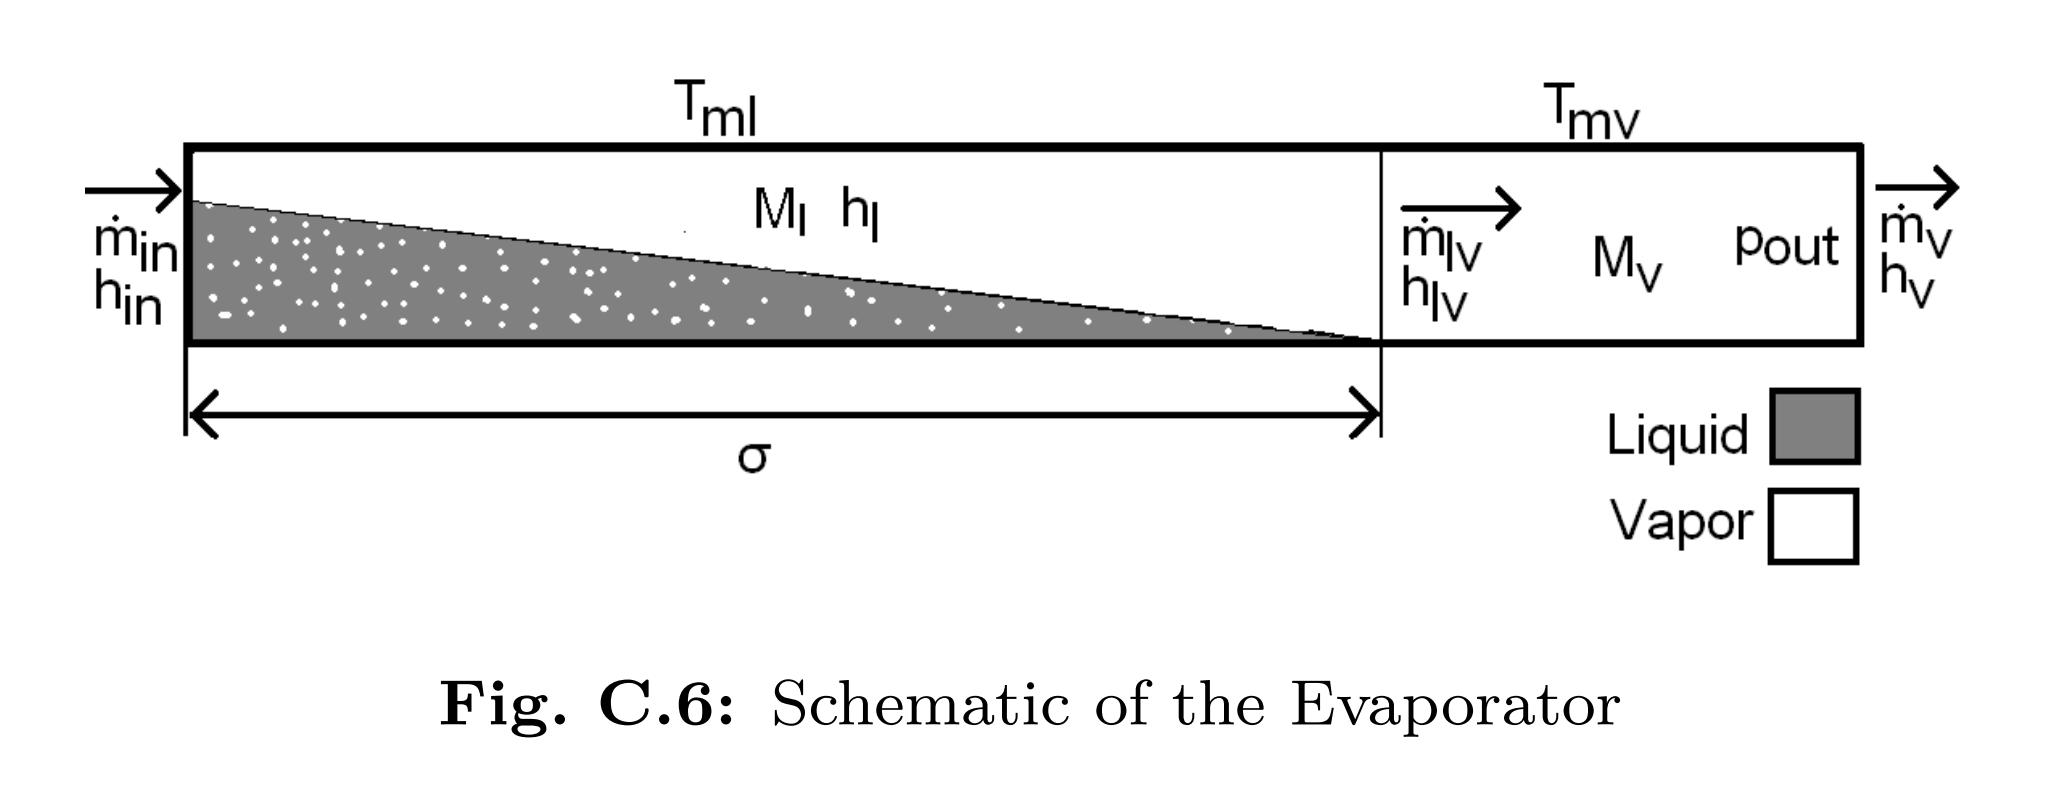
\includegraphics[width=0.6\textwidth]{Graphics/evaporator_CV_stolen.jpeg}
	\caption{Stolen evaporator CV diagram \cite{Sorensen2013}}
	\label{fig:evapo_CV}
\end{figure}






The calculation of the boundary location 
\begin{equation}
	\sigma = \frac{M_l \cdot v_1}{V_i}
\end{equation}

\begin{center}
	\begin{tabular}{l p{8cm} l}
		$\sigma$				& Control Volume boundary 			& [$\cdot$] \\		
		$M_l$				& Mass of liquid-vapor CV 			& [\si{kg}] \\		
		$v_1$				& Refrigerant specific volume of vapor-liquid CV	& [$\si{m}^3/\si{kg}$] \\		
		$V_i$				& Evaporator volume 			& [$\si{m}^3$]
	\end{tabular}
\end{center}


where


Another set of equations:
\begin{align}
	Q_{fan} 		& = (155 \cdot U_{fan}^2 + 40 \cdot U_{fan}^3) \cdot 0.2 \\
	T_{retfan} 		& = T_{ret} + \frac{Q_{fan}}{\dot{m_{air}} \cdot Cp_{air}} \\
	Q_{amv} 		& = Cp_{air} \cdot \dot{m_{air}} \cdot (T_{retfan} - T_{mv}) \\
	T_{retsh} 		& = T_{retfan} - \frac{Q_{amv}}{\dot{m_{air}} \dot Cp_{air}} \\
	Q_{aml} 		& = Cp_{air} \cdot \dot{m_{air}} \cdot (T_{retsh} - T_{ml}) \\
	Q_{mvml} 		& = U A_3 \cdot (T_{mv} - T_{ml}) \\
	Q_{ml} 			& = U A_1 \cdot (T_{ml} - T_l) \cdot \sigma\\
	Q_{mv} 			& = U A_2 \cdot (T_{mv} - T_v) \cdot (1- \sigma)
\end{align}
where
XXX

The airflow over the evaporator is xxxx this behaviour is modeled by:

\begin{align}
	\bar{\dot{m_{air}}} & = \frac{U_{fan}^2 \cdot 3400.5 + U_{fan}^3 \cdot -1103.5} {3600 \cdot \rho_{air}}
	\frac{\Delta \dot{m_{air}}}{\Delta t} & = \frac{\bar{\dot{m_{air}}} - \dot{m_{air}}} {10s}
\end{align}

where

The remaining state equations are given by equations:

\begin{align}
	\frac{dT_{ml}}{dt} & = \frac{Q_{aml}-Q_{ml} + Q_{mvml}}{M_m \cdot Cp_m \cdot \sigma} \\
	\frac{dT_{mv}}{dt} & = \frac{Q_{amv} - Q_{mv} - Q_{mvml}}{M_m \cdot Cp_m \cdot (1- \sigma)} \\
	p_out & = PHV \left( h_v, \frac{V_i-V_l}{M_v} \right)\\
	h_l & = H_{in} + \frac{q_{ml}}{\dot{m_{in}}}\\
	h_v & = H_{lv} + \frac{Q_{mv}}{\dot{m_{lv}}}\\
	\frac{dM_l}{dt} & = \dot{m_{in}} - \dot{m_{lv}}\\
	\frac{DM_v}{dt} & = \dot{m_{lv}} - \dot{m_{out}}\\
	T_{sup} & = T_{retfan} +  \frac{Q_{aml} + A_{amv}}{CP_{air} \cdot \dot{m_{air}}}
\end{align}

where

The mass flow between the two volumes is given by:
\begin{equation}
	\dot{m_{lv}} = \frac{A_{ml}}{h_{dew} - h_{in}}
\end{equation}

where

\subsubsection{Box}

\begin{align}
	\frac{dT_{air}}{dt} & = \frac{Q_{ca} + Q_{aa} + Q_{fa} + Q_{fan} -Q_{cool}}{M_{air} \cdot Cp{air}} \\
	\frac{dT_{floor}}{dt} & = \frac{Q_{af} - Q_{fa}}{M_{floor} \cdot Cp_{floor}} \\
	\frac{dT_{cargo}}{dt} & = \frac{-Q_{ca}}{M_{cargo} \cdot Cp_{cargo}}
\end{align}

where

The temperature difference between the return and supply temperature:

\begin{align}
	Q_{cool} & = Cp_{air} \cdot \dot{m_{air}} \cdot (T_{ret} - T_{sup})\\
	Q_{aa} & = (T_{amp} - T_{air}) \cdot U A_{amp} \cdot 0.81\\
	Q_{af} & = (T_{amp} - T_{floor}) \cdot U A_{amb} \cdot 0.19\\
	Q_{ca} & = (T_{cargo} - T_{air}) \cdot U A_{cargo}\\
	Q_{fa} & = (T_{floor} - T_{air}) \cdot U A_{floor}\\
	Q_{fan} & = (155 \cdot U_{fan}^2 + 40 \cdot U_{fan}^3) \cdot 0.8
\end{align}

where


\subsubsection{Thermodynamic}

\begin{itemize}
	\item Compressor (static) \cite{Sorensen2013} p. 122
	\item Condensor
	\item Reciever
	\item Valve (static) \cite{Sorensen2013} p. 122
	\item Economizer
	\item Evaporator
	\item Pipe joining junction
	\item Pipe splitting junction
	\item Box
\end{itemize}

\subsubsection{Electric}

\begin{itemize}
	\item Battery
	\item Inverter
\end{itemize}

\subsection{Collection of components}

\subsubsection{Linearisation}